\documentclass[1p]{elsarticle_modified}
%\bibliographystyle{elsarticle-num}

%\usepackage[colorlinks]{hyperref}
%\usepackage{abbrmath_seonhwa} %\Abb, \Ascr, \Acal ,\Abf, \Afrak
\usepackage{amsfonts}
\usepackage{amssymb}
\usepackage{amsmath}
\usepackage{amsthm}
\usepackage{scalefnt}
\usepackage{amsbsy}
\usepackage{kotex}
\usepackage{caption}
\usepackage{subfig}
\usepackage{color}
\usepackage{graphicx}
\usepackage{xcolor} %% white, black, red, green, blue, cyan, magenta, yellow
\usepackage{float}
\usepackage{setspace}
\usepackage{hyperref}

\usepackage{tikz}
\usetikzlibrary{arrows}

\usepackage{multirow}
\usepackage{array} % fixed length table
\usepackage{hhline}

%%%%%%%%%%%%%%%%%%%%%
\makeatletter
\renewcommand*\env@matrix[1][\arraystretch]{%
	\edef\arraystretch{#1}%
	\hskip -\arraycolsep
	\let\@ifnextchar\new@ifnextchar
	\array{*\c@MaxMatrixCols c}}
\makeatother %https://tex.stackexchange.com/questions/14071/how-can-i-increase-the-line-spacing-in-a-matrix
%%%%%%%%%%%%%%%

\usepackage[normalem]{ulem}

\newcommand{\msout}[1]{\ifmmode\text{\sout{\ensuremath{#1}}}\else\sout{#1}\fi}
%SOURCE: \msout is \stkout macro in https://tex.stackexchange.com/questions/20609/strikeout-in-math-mode

\newcommand{\cancel}[1]{
	\ifmmode
	{\color{red}\msout{#1}}
	\else
	{\color{red}\sout{#1}}
	\fi
}

\newcommand{\add}[1]{
	{\color{blue}\uwave{#1}}
}

\newcommand{\replace}[2]{
	\ifmmode
	{\color{red}\msout{#1}}{\color{blue}\uwave{#2}}
	\else
	{\color{red}\sout{#1}}{\color{blue}\uwave{#2}}
	\fi
}

\newcommand{\Sol}{\mathcal{S}} %segment
\newcommand{\D}{D} %diagram
\newcommand{\A}{\mathcal{A}} %arc


%%%%%%%%%%%%%%%%%%%%%%%%%%%%%5 test

\def\sl{\operatorname{\textup{SL}}(2,\Cbb)}
\def\psl{\operatorname{\textup{PSL}}(2,\Cbb)}
\def\quan{\mkern 1mu \triangleright \mkern 1mu}

\theoremstyle{definition}
\newtheorem{thm}{Theorem}[section]
\newtheorem{prop}[thm]{Proposition}
\newtheorem{lem}[thm]{Lemma}
\newtheorem{ques}[thm]{Question}
\newtheorem{cor}[thm]{Corollary}
\newtheorem{defn}[thm]{Definition}
\newtheorem{exam}[thm]{Example}
\newtheorem{rmk}[thm]{Remark}
\newtheorem{alg}[thm]{Algorithm}

\newcommand{\I}{\sqrt{-1}}
\begin{document}

%\begin{frontmatter}
%
%\title{Boundary parabolic representations of knots up to 8 crossings}
%
%%% Group authors per affiliation:
%\author{Yunhi Cho} 
%\address{Department of Mathematics, University of Seoul, Seoul, Korea}
%\ead{yhcho@uos.ac.kr}
%
%
%\author{Seonhwa Kim} %\fnref{s_kim}}
%\address{Center for Geometry and Physics, Institute for Basic Science, Pohang, 37673, Korea}
%\ead{ryeona17@ibs.re.kr}
%
%\author{Hyuk Kim}
%\address{Department of Mathematical Sciences, Seoul National University, Seoul 08826, Korea}
%\ead{hyukkim@snu.ac.kr}
%
%\author{Seokbeom Yoon}
%\address{Department of Mathematical Sciences, Seoul National University, Seoul, 08826,  Korea}
%\ead{sbyoon15@snu.ac.kr}
%
%\begin{abstract}
%We find all boundary parabolic representation of knots up to 8 crossings.
%
%\end{abstract}
%\begin{keyword}
%    \MSC[2010] 57M25 
%\end{keyword}
%
%\end{frontmatter}

%\linenumbers
%\tableofcontents
%
\newcommand\colored[1]{\textcolor{white}{\rule[-0.35ex]{0.8em}{1.4ex}}\kern-0.8em\color{red} #1}%
%\newcommand\colored[1]{\textcolor{white}{ #1}\kern-2.17ex	\textcolor{white}{ #1}\kern-1.81ex	\textcolor{white}{ #1}\kern-2.15ex\color{red}#1	}

{\Large $\underline{12n_{0158}~(K12n_{0158})}$}

\setlength{\tabcolsep}{10pt}
\renewcommand{\arraystretch}{1.6}
\vspace{1cm}\begin{tabular}{m{100pt}>{\centering\arraybackslash}m{274pt}}
\multirow{5}{120pt}{
	\centering
	\includegraphics[width=112pt]{../../../GIT/diagram.site/Diagrams/png/2247_12n_0158.png}\\
\ \ \ A knot diagram\footnotemark}&
\allowdisplaybreaks
\textbf{Linearized knot diagam} \\
\cline{2-2}
 &
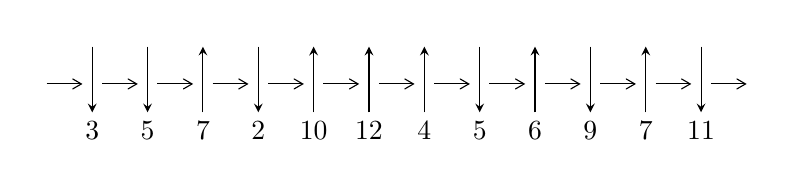
\begin{tikzpicture}[x=20pt, y=17pt]
	% nodes
	\node (C0) at (0, 0) {};
	\node (C1) at (1, 0) {};
	\node (C1U) at (1, +1) {};
	\node (C1D) at (1, -1) {3};

	\node (C2) at (2, 0) {};
	\node (C2U) at (2, +1) {};
	\node (C2D) at (2, -1) {5};

	\node (C3) at (3, 0) {};
	\node (C3U) at (3, +1) {};
	\node (C3D) at (3, -1) {7};

	\node (C4) at (4, 0) {};
	\node (C4U) at (4, +1) {};
	\node (C4D) at (4, -1) {2};

	\node (C5) at (5, 0) {};
	\node (C5U) at (5, +1) {};
	\node (C5D) at (5, -1) {10};

	\node (C6) at (6, 0) {};
	\node (C6U) at (6, +1) {};
	\node (C6D) at (6, -1) {12};

	\node (C7) at (7, 0) {};
	\node (C7U) at (7, +1) {};
	\node (C7D) at (7, -1) {4};

	\node (C8) at (8, 0) {};
	\node (C8U) at (8, +1) {};
	\node (C8D) at (8, -1) {5};

	\node (C9) at (9, 0) {};
	\node (C9U) at (9, +1) {};
	\node (C9D) at (9, -1) {6};

	\node (C10) at (10, 0) {};
	\node (C10U) at (10, +1) {};
	\node (C10D) at (10, -1) {9};

	\node (C11) at (11, 0) {};
	\node (C11U) at (11, +1) {};
	\node (C11D) at (11, -1) {7};

	\node (C12) at (12, 0) {};
	\node (C12U) at (12, +1) {};
	\node (C12D) at (12, -1) {11};
	\node (C13) at (13, 0) {};

	% arrows
	\draw[->,>={angle 60}]
	(C0) edge (C1) (C1) edge (C2) (C2) edge (C3) (C3) edge (C4) (C4) edge (C5) (C5) edge (C6) (C6) edge (C7) (C7) edge (C8) (C8) edge (C9) (C9) edge (C10) (C10) edge (C11) (C11) edge (C12) (C12) edge (C13) ;	\draw[->,>=stealth]
	(C1U) edge (C1D) (C2U) edge (C2D) (C3D) edge (C3U) (C4U) edge (C4D) (C5D) edge (C5U) (C6D) edge (C6U) (C7D) edge (C7U) (C8U) edge (C8D) (C9D) edge (C9U) (C10U) edge (C10D) (C11D) edge (C11U) (C12U) edge (C12D) ;
	\end{tikzpicture} \\
\hhline{~~} \\& 
\textbf{Solving Sequence} \\ \cline{2-2} 
 &
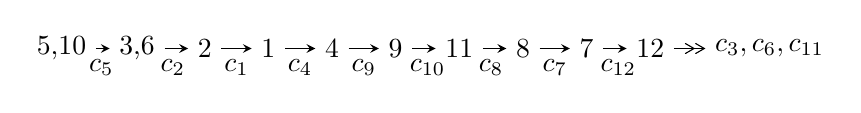
\begin{tikzpicture}[x=23pt, y=7pt]
	% node
	\node (A0) at (-1/8, 0) {5,10};
	\node (A1) at (17/16, 0) {3,6};
	\node (A2) at (17/8, 0) {2};
	\node (A3) at (25/8, 0) {1};
	\node (A4) at (33/8, 0) {4};
	\node (A5) at (41/8, 0) {9};
	\node (A6) at (49/8, 0) {11};
	\node (A7) at (57/8, 0) {8};
	\node (A8) at (65/8, 0) {7};
	\node (A9) at (73/8, 0) {12};
	\node (C1) at (1/2, -1) {$c_{5}$};
	\node (C2) at (13/8, -1) {$c_{2}$};
	\node (C3) at (21/8, -1) {$c_{1}$};
	\node (C4) at (29/8, -1) {$c_{4}$};
	\node (C5) at (37/8, -1) {$c_{9}$};
	\node (C6) at (45/8, -1) {$c_{10}$};
	\node (C7) at (53/8, -1) {$c_{8}$};
	\node (C8) at (61/8, -1) {$c_{7}$};
	\node (C9) at (69/8, -1) {$c_{12}$};
	\node (A10) at (11, 0) {$c_{3},c_{6},c_{11}$};

	% edge
	\draw[->,>=stealth]	
	(A0) edge (A1) (A1) edge (A2) (A2) edge (A3) (A3) edge (A4) (A4) edge (A5) (A5) edge (A6) (A6) edge (A7) (A7) edge (A8) (A8) edge (A9) ;
	\draw[->>,>={angle 60}]	
	(A9) edge (A10);
\end{tikzpicture} \\ 

\end{tabular} \\

\footnotetext{
The image of knot diagram is generated by the software ``\textbf{Draw programme}" developed by Andrew Bartholomew(\url{http://www.layer8.co.uk/maths/draw/index.htm\#Running-draw}), where we modified some parts for our purpose(\url{https://github.com/CATsTAILs/LinksPainter}).
}\phantom \\ \newline 
\centering \textbf{Ideals for irreducible components\footnotemark of $X_{\text{par}}$} 
 
\begin{align*}
I^u_{1}&=\langle 
37 u^{25}+5 u^{24}+\cdots+32 b+3,\;11 u^{25}- u^{24}+\cdots+64 a+73,\;u^{26}+5 u^{24}+\cdots+7 u^2+1\rangle \\
I^u_{2}&=\langle 
1.64036\times10^{19} u^{35}-6.55779\times10^{19} u^{34}+\cdots+1.64861\times10^{20} b-8.76883\times10^{20},\\
\phantom{I^u_{2}}&\phantom{= \langle  }-2.73439\times10^{20} u^{35}+9.88504\times10^{20} u^{34}+\cdots+2.80263\times10^{21} a+2.34140\times10^{22},\\
\phantom{I^u_{2}}&\phantom{= \langle  }u^{36}-2 u^{35}+\cdots-16 u+17\rangle \\
I^u_{3}&=\langle 
b+1,\;- u^3+u^2+2 a+1,\;u^4+u^2+u+1\rangle \\
I^u_{4}&=\langle 
b+1,\;u^5- u^4+u^3- u^2+a+u,\;u^6- u^5+2 u^4-2 u^3+2 u^2-2 u+1\rangle \\
I^u_{5}&=\langle 
- a^2+2 a u+b+2 a-2 u-1,\;a^3-3 a^2 u-3 a^2+6 a u+a-2 u+1,\;u^2+1\rangle \\
\\
\end{align*}
\raggedright * 5 irreducible components of $\dim_{\mathbb{C}}=0$, with total 78 representations.\\
\footnotetext{All coefficients of polynomials are rational numbers. But the coefficients are sometimes approximated in decimal forms when there is not enough margin.}
\newpage
\renewcommand{\arraystretch}{1}
\centering \section*{I. $I^u_{1}= \langle 37 u^{25}+5 u^{24}+\cdots+32 b+3,\;11 u^{25}- u^{24}+\cdots+64 a+73,\;u^{26}+5 u^{24}+\cdots+7 u^2+1 \rangle$}
\flushleft \textbf{(i) Arc colorings}\\
\begin{tabular}{m{7pt} m{180pt} m{7pt} m{180pt} }
\flushright $a_{5}=$&$\begin{pmatrix}1\\0\end{pmatrix}$ \\
\flushright $a_{10}=$&$\begin{pmatrix}0\\u\end{pmatrix}$ \\
\flushright $a_{3}=$&$\begin{pmatrix}-0.171875 u^{25}+0.0156250 u^{24}+\cdots+4.29688 u-1.14063\\-1.15625 u^{25}-0.156250 u^{24}+\cdots-1.59375 u-0.0937500\end{pmatrix}$ \\
\flushright $a_{6}=$&$\begin{pmatrix}1\\- u^2\end{pmatrix}$ \\
\flushright $a_{2}=$&$\begin{pmatrix}-1.32813 u^{25}-0.140625 u^{24}+\cdots+2.70313 u-1.23438\\-1.15625 u^{25}-0.156250 u^{24}+\cdots-1.59375 u-0.0937500\end{pmatrix}$ \\
\flushright $a_{1}=$&$\begin{pmatrix}\frac{1}{8} u^{24}+\frac{1}{2} u^{22}+\cdots+u+\frac{1}{8}\\\frac{1}{8} u^{24}+\frac{1}{2} u^{22}+\cdots+u+\frac{1}{8}\end{pmatrix}$ \\
\flushright $a_{4}=$&$\begin{pmatrix}1.39063 u^{25}+0.203125 u^{24}+\cdots+4.48438 u-2.07813\\0.593750 u^{25}+0.343750 u^{24}+\cdots-0.0937500 u-0.593750\end{pmatrix}$ \\
\flushright $a_{9}=$&$\begin{pmatrix}- u\\u^3+u\end{pmatrix}$ \\
\flushright $a_{11}=$&$\begin{pmatrix}- u^3\\u^5+u^3+u\end{pmatrix}$ \\
\flushright $a_{8}=$&$\begin{pmatrix}u^3\\u^3+u\end{pmatrix}$ \\
\flushright $a_{7}=$&$\begin{pmatrix}\frac{1}{8} u^{25}+\frac{1}{2} u^{23}+\cdots+\frac{1}{8} u-1\\\frac{1}{8} u^{25}+\frac{1}{2} u^{23}+\cdots+2 u^2+\frac{1}{8} u\end{pmatrix}$ \\
\flushright $a_{12}=$&$\begin{pmatrix}\frac{1}{8} u^{24}+\frac{1}{2} u^{22}+\cdots+u+\frac{1}{8}\\\frac{1}{8} u^{24}+\frac{1}{2} u^{22}+\cdots+u+\frac{1}{8}\end{pmatrix}$\\&\end{tabular}
\flushleft \textbf{(ii) Obstruction class $= -1$}\\~\\
\flushleft \textbf{(iii) Cusp Shapes $= -\frac{563}{128} u^{25}-\frac{159}{128} u^{24}+\cdots-\frac{1045}{128} u-\frac{521}{128}$}\\~\\
\newpage\renewcommand{\arraystretch}{1}
\flushleft \textbf{(iv) u-Polynomials at the component}\newline \\
\begin{tabular}{m{50pt}|m{274pt}}
Crossings & \hspace{64pt}u-Polynomials at each crossing \\
\hline $$\begin{aligned}c_{1}\end{aligned}$$&$\begin{aligned}
&u^{26}+7 u^{25}+\cdots-47 u+16
\end{aligned}$\\
\hline $$\begin{aligned}c_{2},c_{4}\end{aligned}$$&$\begin{aligned}
&u^{26}-5 u^{25}+\cdots-17 u+4
\end{aligned}$\\
\hline $$\begin{aligned}c_{3},c_{7}\end{aligned}$$&$\begin{aligned}
&u^{26}-3 u^{25}+\cdots-304 u+64
\end{aligned}$\\
\hline $$\begin{aligned}c_{5},c_{6},c_{9}\\c_{11}\end{aligned}$$&$\begin{aligned}
&u^{26}+5 u^{24}+\cdots+7 u^2+1
\end{aligned}$\\
\hline $$\begin{aligned}c_{8}\end{aligned}$$&$\begin{aligned}
&u^{26}+6 u^{25}+\cdots+1024 u+256
\end{aligned}$\\
\hline $$\begin{aligned}c_{10},c_{12}\end{aligned}$$&$\begin{aligned}
&u^{26}+10 u^{25}+\cdots+14 u+1
\end{aligned}$\\
\hline
\end{tabular}\\~\\
\newpage\renewcommand{\arraystretch}{1}
\flushleft \textbf{(v) Riley Polynomials at the component}\newline \\
\begin{tabular}{m{50pt}|m{274pt}}
Crossings & \hspace{64pt}Riley Polynomials at each crossing \\
\hline $$\begin{aligned}c_{1}\end{aligned}$$&$\begin{aligned}
&y^{26}+29 y^{25}+\cdots-4769 y+256
\end{aligned}$\\
\hline $$\begin{aligned}c_{2},c_{4}\end{aligned}$$&$\begin{aligned}
&y^{26}-7 y^{25}+\cdots+47 y+16
\end{aligned}$\\
\hline $$\begin{aligned}c_{3},c_{7}\end{aligned}$$&$\begin{aligned}
&y^{26}-27 y^{25}+\cdots-28928 y+4096
\end{aligned}$\\
\hline $$\begin{aligned}c_{5},c_{6},c_{9}\\c_{11}\end{aligned}$$&$\begin{aligned}
&y^{26}+10 y^{25}+\cdots+14 y+1
\end{aligned}$\\
\hline $$\begin{aligned}c_{8}\end{aligned}$$&$\begin{aligned}
&y^{26}+10 y^{25}+\cdots+1540096 y+65536
\end{aligned}$\\
\hline $$\begin{aligned}c_{10},c_{12}\end{aligned}$$&$\begin{aligned}
&y^{26}+22 y^{25}+\cdots+22 y+1
\end{aligned}$\\
\hline
\end{tabular}\\~\\
\newpage\flushleft \textbf{(vi) Complex Volumes and Cusp Shapes}
$$\begin{array}{c|c|c}  
\text{Solutions to }I^u_{1}& \I (\text{vol} + \sqrt{-1}CS) & \text{Cusp shape}\\
 \hline 
\begin{aligned}
u &= \phantom{-}0.686718 + 0.790237 I \\
a &= \phantom{-}0.862776 + 0.752523 I \\
b &= -0.112686 - 0.757455 I\end{aligned}
 & \phantom{-}1.98398 + 2.27305 I & \phantom{-}3.49441 - 2.95209 I \\ \hline\begin{aligned}
u &= \phantom{-}0.686718 - 0.790237 I \\
a &= \phantom{-}0.862776 - 0.752523 I \\
b &= -0.112686 + 0.757455 I\end{aligned}
 & \phantom{-}1.98398 - 2.27305 I & \phantom{-}3.49441 + 2.95209 I \\ \hline\begin{aligned}
u &= \phantom{-}0.332646 + 0.885585 I \\
a &= \phantom{-}0.859182 + 0.253751 I \\
b &= \phantom{-}0.966203 + 0.651765 I\end{aligned}
 & \phantom{-}0.374508 - 1.260680 I & \phantom{-}0.03372 - 2.82297 I \\ \hline\begin{aligned}
u &= \phantom{-}0.332646 - 0.885585 I \\
a &= \phantom{-}0.859182 - 0.253751 I \\
b &= \phantom{-}0.966203 - 0.651765 I\end{aligned}
 & \phantom{-}0.374508 + 1.260680 I & \phantom{-}0.03372 + 2.82297 I \\ \hline\begin{aligned}
u &= -0.943048 + 0.573575 I \\
a &= -0.572959 + 1.084400 I \\
b &= \phantom{-}1.06906 - 0.99419 I\end{aligned}
 & \phantom{-}9.87605 + 3.35816 I & \phantom{-}3.98629 - 0.41980 I \\ \hline\begin{aligned}
u &= -0.943048 - 0.573575 I \\
a &= -0.572959 - 1.084400 I \\
b &= \phantom{-}1.06906 + 0.99419 I\end{aligned}
 & \phantom{-}9.87605 - 3.35816 I & \phantom{-}3.98629 + 0.41980 I \\ \hline\begin{aligned}
u &= -0.597517 + 0.932496 I \\
a &= -0.074973 - 0.361234 I \\
b &= -1.085400 + 0.468804 I\end{aligned}
 & -1.78026 - 3.46737 I & -1.87106 + 4.78330 I \\ \hline\begin{aligned}
u &= -0.597517 - 0.932496 I \\
a &= -0.074973 + 0.361234 I \\
b &= -1.085400 - 0.468804 I\end{aligned}
 & -1.78026 + 3.46737 I & -1.87106 - 4.78330 I \\ \hline\begin{aligned}
u &= -0.925240 + 0.681323 I \\
a &= -0.07111 - 1.54316 I \\
b &= \phantom{-}0.94455 + 1.07986 I\end{aligned}
 & \phantom{-}10.29890 - 4.17338 I & \phantom{-}4.09194 + 4.29853 I \\ \hline\begin{aligned}
u &= -0.925240 - 0.681323 I \\
a &= -0.07111 + 1.54316 I \\
b &= \phantom{-}0.94455 - 1.07986 I\end{aligned}
 & \phantom{-}10.29890 + 4.17338 I & \phantom{-}4.09194 - 4.29853 I\\
 \hline 
 \end{array}$$\newpage$$\begin{array}{c|c|c}  
\text{Solutions to }I^u_{1}& \I (\text{vol} + \sqrt{-1}CS) & \text{Cusp shape}\\
 \hline 
\begin{aligned}
u &= \phantom{-}0.615881 + 1.015000 I \\
a &= -1.05911 - 1.42400 I \\
b &= -1.324650 + 0.202541 I\end{aligned}
 & -2.47670 + 6.15727 I & -1.31624 - 5.25780 I \\ \hline\begin{aligned}
u &= \phantom{-}0.615881 - 1.015000 I \\
a &= -1.05911 + 1.42400 I \\
b &= -1.324650 - 0.202541 I\end{aligned}
 & -2.47670 - 6.15727 I & -1.31624 + 5.25780 I \\ \hline\begin{aligned}
u &= \phantom{-}0.213984 + 0.755898 I \\
a &= \phantom{-}1.343350 + 0.180099 I \\
b &= \phantom{-}0.844053 - 0.643735 I\end{aligned}
 & \phantom{-}0.79107 + 3.73974 I & \phantom{-}2.88234 - 8.52096 I \\ \hline\begin{aligned}
u &= \phantom{-}0.213984 - 0.755898 I \\
a &= \phantom{-}1.343350 - 0.180099 I \\
b &= \phantom{-}0.844053 + 0.643735 I\end{aligned}
 & \phantom{-}0.79107 - 3.73974 I & \phantom{-}2.88234 + 8.52096 I \\ \hline\begin{aligned}
u &= -0.522459 + 1.135990 I \\
a &= \phantom{-}1.068060 - 0.495553 I \\
b &= \phantom{-}0.679614 + 0.169964 I\end{aligned}
 & -3.56752 - 8.00011 I & \phantom{-}1.95259 + 8.91191 I \\ \hline\begin{aligned}
u &= -0.522459 - 1.135990 I \\
a &= \phantom{-}1.068060 + 0.495553 I \\
b &= \phantom{-}0.679614 - 0.169964 I\end{aligned}
 & -3.56752 + 8.00011 I & \phantom{-}1.95259 - 8.91191 I \\ \hline\begin{aligned}
u &= -0.661950 + 1.073520 I \\
a &= -0.360539 + 1.342880 I \\
b &= -0.585613 - 0.805144 I\end{aligned}
 & \phantom{-}0.06912 - 8.45528 I & -0.31615 + 7.82627 I \\ \hline\begin{aligned}
u &= -0.661950 - 1.073520 I \\
a &= -0.360539 - 1.342880 I \\
b &= -0.585613 + 0.805144 I\end{aligned}
 & \phantom{-}0.06912 + 8.45528 I & -0.31615 - 7.82627 I \\ \hline\begin{aligned}
u &= \phantom{-}0.573105 + 0.355043 I \\
a &= \phantom{-}0.431069 - 0.470281 I \\
b &= \phantom{-}0.145218 + 0.443676 I\end{aligned}
 & \phantom{-}1.181070 + 0.652752 I & \phantom{-}6.65549 - 2.84470 I \\ \hline\begin{aligned}
u &= \phantom{-}0.573105 - 0.355043 I \\
a &= \phantom{-}0.431069 + 0.470281 I \\
b &= \phantom{-}0.145218 - 0.443676 I\end{aligned}
 & \phantom{-}1.181070 - 0.652752 I & \phantom{-}6.65549 + 2.84470 I\\
 \hline 
 \end{array}$$\newpage$$\begin{array}{c|c|c}  
\text{Solutions to }I^u_{1}& \I (\text{vol} + \sqrt{-1}CS) & \text{Cusp shape}\\
 \hline 
\begin{aligned}
u &= \phantom{-}0.715044 + 1.157990 I \\
a &= -0.890942 - 0.102027 I \\
b &= \phantom{-}0.750500 + 1.133340 I\end{aligned}
 & \phantom{-}7.16363 + 8.23028 I & \phantom{-}1.13390 - 4.65943 I \\ \hline\begin{aligned}
u &= \phantom{-}0.715044 - 1.157990 I \\
a &= -0.890942 + 0.102027 I \\
b &= \phantom{-}0.750500 - 1.133340 I\end{aligned}
 & \phantom{-}7.16363 - 8.23028 I & \phantom{-}1.13390 + 4.65943 I \\ \hline\begin{aligned}
u &= \phantom{-}0.674140 + 1.197450 I \\
a &= \phantom{-}1.10131 + 1.68297 I \\
b &= \phantom{-}1.16977 - 0.88449 I\end{aligned}
 & \phantom{-}5.7894 + 15.5253 I & -0.62931 - 8.80838 I \\ \hline\begin{aligned}
u &= \phantom{-}0.674140 - 1.197450 I \\
a &= \phantom{-}1.10131 - 1.68297 I \\
b &= \phantom{-}1.16977 + 0.88449 I\end{aligned}
 & \phantom{-}5.7894 - 15.5253 I & -0.62931 + 8.80838 I \\ \hline\begin{aligned}
u &= -0.161303 + 0.352465 I \\
a &= -0.88611 + 2.09278 I \\
b &= -0.960623 - 0.194500 I\end{aligned}
 & -1.73934 - 0.69423 I & -4.47291 + 0.47105 I \\ \hline\begin{aligned}
u &= -0.161303 - 0.352465 I \\
a &= -0.88611 - 2.09278 I \\
b &= -0.960623 + 0.194500 I\end{aligned}
 & -1.73934 + 0.69423 I & -4.47291 - 0.47105 I\\
 \hline 
 \end{array}$$\newpage\newpage\renewcommand{\arraystretch}{1}
\centering \section*{II. $I^u_{2}= \langle 1.64\times10^{19} u^{35}-6.56\times10^{19} u^{34}+\cdots+1.65\times10^{20} b-8.77\times10^{20},\;-2.73\times10^{20} u^{35}+9.89\times10^{20} u^{34}+\cdots+2.80\times10^{21} a+2.34\times10^{22},\;u^{36}-2 u^{35}+\cdots-16 u+17 \rangle$}
\flushleft \textbf{(i) Arc colorings}\\
\begin{tabular}{m{7pt} m{180pt} m{7pt} m{180pt} }
\flushright $a_{5}=$&$\begin{pmatrix}1\\0\end{pmatrix}$ \\
\flushright $a_{10}=$&$\begin{pmatrix}0\\u\end{pmatrix}$ \\
\flushright $a_{3}=$&$\begin{pmatrix}0.0975652 u^{35}-0.352706 u^{34}+\cdots+2.60900 u-8.35431\\-0.0994997 u^{35}+0.397778 u^{34}+\cdots-0.756708 u+5.31894\end{pmatrix}$ \\
\flushright $a_{6}=$&$\begin{pmatrix}1\\- u^2\end{pmatrix}$ \\
\flushright $a_{2}=$&$\begin{pmatrix}-0.00193454 u^{35}+0.0450723 u^{34}+\cdots+1.85229 u-3.03538\\-0.0994997 u^{35}+0.397778 u^{34}+\cdots-0.756708 u+5.31894\end{pmatrix}$ \\
\flushright $a_{1}=$&$\begin{pmatrix}0.167671 u^{35}-0.201737 u^{34}+\cdots+7.20414 u-0.801787\\-0.203086 u^{35}+0.207511 u^{34}+\cdots-4.38662 u+1.19177\end{pmatrix}$ \\
\flushright $a_{4}=$&$\begin{pmatrix}-0.677695 u^{35}+1.09907 u^{34}+\cdots-8.59244 u+5.59975\\0.0381892 u^{35}-0.396278 u^{34}+\cdots+0.00858699 u-5.74660\end{pmatrix}$ \\
\flushright $a_{9}=$&$\begin{pmatrix}- u\\u^3+u\end{pmatrix}$ \\
\flushright $a_{11}=$&$\begin{pmatrix}- u^3\\u^5+u^3+u\end{pmatrix}$ \\
\flushright $a_{8}=$&$\begin{pmatrix}u^3\\u^3+u\end{pmatrix}$ \\
\flushright $a_{7}=$&$\begin{pmatrix}-0.0123763 u^{35}+0.0202099 u^{34}+\cdots+1.02313 u+3.72869\\0.0511253 u^{35}-0.134072 u^{34}+\cdots+0.364967 u-2.38667\end{pmatrix}$ \\
\flushright $a_{12}=$&$\begin{pmatrix}0.135850 u^{35}-0.216397 u^{34}+\cdots+6.63547 u-1.67092\\-0.158595 u^{35}+0.210763 u^{34}+\cdots-1.68145 u+1.66988\end{pmatrix}$\\&\end{tabular}
\flushleft \textbf{(ii) Obstruction class $= -1$}\\~\\
\flushleft \textbf{(iii) Cusp Shapes $= -\frac{92294208925977637035}{164860561334912795863} u^{35}+\frac{248194929627859910457}{164860561334912795863} u^{34}+\cdots-\frac{1193076869772129210292}{164860561334912795863} u+\frac{1468116381237737523006}{164860561334912795863}$}\\~\\
\newpage\renewcommand{\arraystretch}{1}
\flushleft \textbf{(iv) u-Polynomials at the component}\newline \\
\begin{tabular}{m{50pt}|m{274pt}}
Crossings & \hspace{64pt}u-Polynomials at each crossing \\
\hline $$\begin{aligned}c_{1}\end{aligned}$$&$\begin{aligned}
&(u^{18}+4 u^{17}+\cdots+11 u+1)^{2}
\end{aligned}$\\
\hline $$\begin{aligned}c_{2},c_{4}\end{aligned}$$&$\begin{aligned}
&(u^{18}-4 u^{17}+\cdots+3 u-1)^{2}
\end{aligned}$\\
\hline $$\begin{aligned}c_{3},c_{7}\end{aligned}$$&$\begin{aligned}
&(u^{18}+u^{17}+\cdots+4 u+8)^{2}
\end{aligned}$\\
\hline $$\begin{aligned}c_{5},c_{6},c_{9}\\c_{11}\end{aligned}$$&$\begin{aligned}
&u^{36}-2 u^{35}+\cdots-16 u+17
\end{aligned}$\\
\hline $$\begin{aligned}c_{8}\end{aligned}$$&$\begin{aligned}
&(u^{18}-2 u^{17}+\cdots-18 u-17)^{2}
\end{aligned}$\\
\hline $$\begin{aligned}c_{10},c_{12}\end{aligned}$$&$\begin{aligned}
&u^{36}+18 u^{35}+\cdots+1784 u+289
\end{aligned}$\\
\hline
\end{tabular}\\~\\
\newpage\renewcommand{\arraystretch}{1}
\flushleft \textbf{(v) Riley Polynomials at the component}\newline \\
\begin{tabular}{m{50pt}|m{274pt}}
Crossings & \hspace{64pt}Riley Polynomials at each crossing \\
\hline $$\begin{aligned}c_{1}\end{aligned}$$&$\begin{aligned}
&(y^{18}+24 y^{17}+\cdots-11 y+1)^{2}
\end{aligned}$\\
\hline $$\begin{aligned}c_{2},c_{4}\end{aligned}$$&$\begin{aligned}
&(y^{18}-4 y^{17}+\cdots-11 y+1)^{2}
\end{aligned}$\\
\hline $$\begin{aligned}c_{3},c_{7}\end{aligned}$$&$\begin{aligned}
&(y^{18}-21 y^{17}+\cdots-592 y+64)^{2}
\end{aligned}$\\
\hline $$\begin{aligned}c_{5},c_{6},c_{9}\\c_{11}\end{aligned}$$&$\begin{aligned}
&y^{36}+18 y^{35}+\cdots+1784 y+289
\end{aligned}$\\
\hline $$\begin{aligned}c_{8}\end{aligned}$$&$\begin{aligned}
&(y^{18}+10 y^{17}+\cdots-1106 y+289)^{2}
\end{aligned}$\\
\hline $$\begin{aligned}c_{10},c_{12}\end{aligned}$$&$\begin{aligned}
&y^{36}-2 y^{35}+\cdots+426376 y+83521
\end{aligned}$\\
\hline
\end{tabular}\\~\\
\newpage\flushleft \textbf{(vi) Complex Volumes and Cusp Shapes}
$$\begin{array}{c|c|c}  
\text{Solutions to }I^u_{2}& \I (\text{vol} + \sqrt{-1}CS) & \text{Cusp shape}\\
 \hline 
\begin{aligned}
u &= \phantom{-}0.591186 + 0.787704 I \\
a &= -1.56603 - 0.88745 I \\
b &= \phantom{-}0.889957 + 0.956699 I\end{aligned}
 & \phantom{-}2.38234 - 1.09047 I & \phantom{-}0.174080 - 0.422577 I \\ \hline\begin{aligned}
u &= \phantom{-}0.591186 - 0.787704 I \\
a &= -1.56603 + 0.88745 I \\
b &= \phantom{-}0.889957 - 0.956699 I\end{aligned}
 & \phantom{-}2.38234 + 1.09047 I & \phantom{-}0.174080 + 0.422577 I \\ \hline\begin{aligned}
u &= -0.794635 + 0.529818 I \\
a &= \phantom{-}0.753156 - 1.018670 I \\
b &= -0.405572 + 0.756937 I\end{aligned}
 & \phantom{-}1.68246 + 2.95811 I & \phantom{-}2.86830 - 3.60082 I \\ \hline\begin{aligned}
u &= -0.794635 - 0.529818 I \\
a &= \phantom{-}0.753156 + 1.018670 I \\
b &= -0.405572 - 0.756937 I\end{aligned}
 & \phantom{-}1.68246 - 2.95811 I & \phantom{-}2.86830 + 3.60082 I \\ \hline\begin{aligned}
u &= -0.575111 + 0.759119 I \\
a &= -0.73772 + 1.69762 I \\
b &= -1.189210 - 0.282581 I\end{aligned}
 & -1.21564 - 1.22055 I & \phantom{-}0.481280 - 0.071123 I \\ \hline\begin{aligned}
u &= -0.575111 - 0.759119 I \\
a &= -0.73772 - 1.69762 I \\
b &= -1.189210 + 0.282581 I\end{aligned}
 & -1.21564 + 1.22055 I & \phantom{-}0.481280 + 0.071123 I \\ \hline\begin{aligned}
u &= \phantom{-}0.167080 + 1.041030 I \\
a &= -2.61040 - 3.09914 I \\
b &= -1.10588\phantom{ +0.000000I}\end{aligned}
 & -5.41960\phantom{ +0.000000I} & \phantom{-}2.98163 + 0. I\phantom{ +0.000000I} \\ \hline\begin{aligned}
u &= \phantom{-}0.167080 - 1.041030 I \\
a &= -2.61040 + 3.09914 I \\
b &= -1.10588\phantom{ +0.000000I}\end{aligned}
 & -5.41960\phantom{ +0.000000I} & \phantom{-}2.98163 + 0. I\phantom{ +0.000000I} \\ \hline\begin{aligned}
u &= \phantom{-}0.997738 + 0.395002 I \\
a &= -0.292945 - 1.197000 I \\
b &= \phantom{-}1.13145 + 0.93287 I\end{aligned}
 & \phantom{-}8.25713 - 9.46502 I & \phantom{-}2.19641 + 5.12935 I \\ \hline\begin{aligned}
u &= \phantom{-}0.997738 - 0.395002 I \\
a &= -0.292945 + 1.197000 I \\
b &= \phantom{-}1.13145 - 0.93287 I\end{aligned}
 & \phantom{-}8.25713 + 9.46502 I & \phantom{-}2.19641 - 5.12935 I\\
 \hline 
 \end{array}$$\newpage$$\begin{array}{c|c|c}  
\text{Solutions to }I^u_{2}& \I (\text{vol} + \sqrt{-1}CS) & \text{Cusp shape}\\
 \hline 
\begin{aligned}
u &= -0.274534 + 0.872882 I \\
a &= \phantom{-}0.93452 + 2.44113 I \\
b &= -0.509257 - 0.343539 I\end{aligned}
 & -3.86556 - 1.11682 I & -2.38496 + 6.15764 I \\ \hline\begin{aligned}
u &= -0.274534 - 0.872882 I \\
a &= \phantom{-}0.93452 - 2.44113 I \\
b &= -0.509257 + 0.343539 I\end{aligned}
 & -3.86556 + 1.11682 I & -2.38496 - 6.15764 I \\ \hline\begin{aligned}
u &= \phantom{-}0.588697 + 0.917985 I \\
a &= \phantom{-}0.52281 + 2.44549 I \\
b &= \phantom{-}1.023450 - 0.903197 I\end{aligned}
 & \phantom{-}1.96168 + 5.76942 I & -0.89628 - 5.17142 I \\ \hline\begin{aligned}
u &= \phantom{-}0.588697 - 0.917985 I \\
a &= \phantom{-}0.52281 - 2.44549 I \\
b &= \phantom{-}1.023450 + 0.903197 I\end{aligned}
 & \phantom{-}1.96168 - 5.76942 I & -0.89628 + 5.17142 I \\ \hline\begin{aligned}
u &= \phantom{-}0.985654 + 0.488151 I \\
a &= -0.268666 + 1.306090 I \\
b &= \phantom{-}0.841043 - 1.112380 I\end{aligned}
 & \phantom{-}9.21890 - 2.04734 I & \phantom{-}3.38974 + 0.64724 I \\ \hline\begin{aligned}
u &= \phantom{-}0.985654 - 0.488151 I \\
a &= -0.268666 - 1.306090 I \\
b &= \phantom{-}0.841043 + 1.112380 I\end{aligned}
 & \phantom{-}9.21890 + 2.04734 I & \phantom{-}3.38974 - 0.64724 I \\ \hline\begin{aligned}
u &= \phantom{-}0.670337 + 0.891635 I \\
a &= -0.058974 - 1.277660 I \\
b &= -0.405572 + 0.756937 I\end{aligned}
 & \phantom{-}1.68246 + 2.95811 I & \phantom{-}2.86830 - 3.60082 I \\ \hline\begin{aligned}
u &= \phantom{-}0.670337 - 0.891635 I \\
a &= -0.058974 + 1.277660 I \\
b &= -0.405572 - 0.756937 I\end{aligned}
 & \phantom{-}1.68246 - 2.95811 I & \phantom{-}2.86830 + 3.60082 I \\ \hline\begin{aligned}
u &= \phantom{-}0.626901 + 0.585336 I \\
a &= -0.339138 + 0.406991 I \\
b &= -1.189210 - 0.282581 I\end{aligned}
 & -1.21564 - 1.22055 I & \phantom{-}0.481280 - 0.071123 I \\ \hline\begin{aligned}
u &= \phantom{-}0.626901 - 0.585336 I \\
a &= -0.339138 - 0.406991 I \\
b &= -1.189210 + 0.282581 I\end{aligned}
 & -1.21564 + 1.22055 I & \phantom{-}0.481280 + 0.071123 I\\
 \hline 
 \end{array}$$\newpage$$\begin{array}{c|c|c}  
\text{Solutions to }I^u_{2}& \I (\text{vol} + \sqrt{-1}CS) & \text{Cusp shape}\\
 \hline 
\begin{aligned}
u &= \phantom{-}0.453358 + 1.062450 I \\
a &= \phantom{-}1.049730 + 0.489075 I \\
b &= \phantom{-}0.550076 - 0.259421 I\end{aligned}
 & -0.92819 + 3.34376 I & \phantom{-}3.77359 - 4.65236 I \\ \hline\begin{aligned}
u &= \phantom{-}0.453358 - 1.062450 I \\
a &= \phantom{-}1.049730 - 0.489075 I \\
b &= \phantom{-}0.550076 + 0.259421 I\end{aligned}
 & -0.92819 - 3.34376 I & \phantom{-}3.77359 + 4.65236 I \\ \hline\begin{aligned}
u &= -0.106316 + 1.174290 I \\
a &= \phantom{-}0.436208 - 0.085284 I \\
b &= -0.509257 + 0.343539 I\end{aligned}
 & -3.86556 + 1.11682 I & -2.38496 - 6.15764 I \\ \hline\begin{aligned}
u &= -0.106316 - 1.174290 I \\
a &= \phantom{-}0.436208 + 0.085284 I \\
b &= -0.509257 - 0.343539 I\end{aligned}
 & -3.86556 - 1.11682 I & -2.38496 + 6.15764 I \\ \hline\begin{aligned}
u &= -0.331026 + 1.152710 I \\
a &= \phantom{-}0.999190 - 0.535049 I \\
b &= \phantom{-}0.441998\phantom{ +0.000000I}\end{aligned}
 & -4.89262\phantom{ +0.000000I} &                  -6
-1.185937 + 0. 10   I\phantom{ +0.000000I} \\ \hline\begin{aligned}
u &= -0.331026 - 1.152710 I \\
a &= \phantom{-}0.999190 + 0.535049 I \\
b &= \phantom{-}0.441998\phantom{ +0.000000I}\end{aligned}
 & -4.89262\phantom{ +0.000000I} &                  -6
-1.185937 + 0. 10   I\phantom{ +0.000000I} \\ \hline\begin{aligned}
u &= -0.715398 + 0.207958 I \\
a &= \phantom{-}0.433150 - 0.002861 I \\
b &= \phantom{-}0.550076 - 0.259421 I\end{aligned}
 & -0.92819 + 3.34376 I & \phantom{-}3.77359 - 4.65236 I \\ \hline\begin{aligned}
u &= -0.715398 - 0.207958 I \\
a &= \phantom{-}0.433150 + 0.002861 I \\
b &= \phantom{-}0.550076 + 0.259421 I\end{aligned}
 & -0.92819 - 3.34376 I & \phantom{-}3.77359 + 4.65236 I \\ \hline\begin{aligned}
u &= -0.775491 + 1.032570 I \\
a &= -0.952803 + 0.345976 I \\
b &= \phantom{-}0.841043 - 1.112380 I\end{aligned}
 & \phantom{-}9.21890 - 2.04734 I & \phantom{-}3.38974 + 0.64724 I \\ \hline\begin{aligned}
u &= -0.775491 - 1.032570 I \\
a &= -0.952803 - 0.345976 I \\
b &= \phantom{-}0.841043 + 1.112380 I\end{aligned}
 & \phantom{-}9.21890 + 2.04734 I & \phantom{-}3.38974 - 0.64724 I\\
 \hline 
 \end{array}$$\newpage$$\begin{array}{c|c|c}  
\text{Solutions to }I^u_{2}& \I (\text{vol} + \sqrt{-1}CS) & \text{Cusp shape}\\
 \hline 
\begin{aligned}
u &= -0.726810 + 1.099240 I \\
a &= \phantom{-}0.83534 - 1.78440 I \\
b &= \phantom{-}1.13145 + 0.93287 I\end{aligned}
 & \phantom{-}8.25713 - 9.46502 I & \phantom{-}2.19641 + 5.12935 I \\ \hline\begin{aligned}
u &= -0.726810 - 1.099240 I \\
a &= \phantom{-}0.83534 + 1.78440 I \\
b &= \phantom{-}1.13145 - 0.93287 I\end{aligned}
 & \phantom{-}8.25713 + 9.46502 I & \phantom{-}2.19641 - 5.12935 I \\ \hline\begin{aligned}
u &= \phantom{-}0.066926 + 1.357280 I \\
a &= \phantom{-}0.785883 + 0.110703 I \\
b &= \phantom{-}0.889957 - 0.956699 I\end{aligned}
 & \phantom{-}2.38234 + 1.09047 I & \phantom{-}0.174080 + 0.422577 I \\ \hline\begin{aligned}
u &= \phantom{-}0.066926 - 1.357280 I \\
a &= \phantom{-}0.785883 - 0.110703 I \\
b &= \phantom{-}0.889957 + 0.956699 I\end{aligned}
 & \phantom{-}2.38234 - 1.09047 I & \phantom{-}0.174080 - 0.422577 I \\ \hline\begin{aligned}
u &= \phantom{-}0.151444 + 1.368190 I \\
a &= \phantom{-}0.753153 - 0.013270 I \\
b &= \phantom{-}1.023450 + 0.903197 I\end{aligned}
 & \phantom{-}1.96168 - 5.76942 I & -0.89628 + 5.17142 I \\ \hline\begin{aligned}
u &= \phantom{-}0.151444 - 1.368190 I \\
a &= \phantom{-}0.753153 + 0.013270 I \\
b &= \phantom{-}1.023450 - 0.903197 I\end{aligned}
 & \phantom{-}1.96168 + 5.76942 I & -0.89628 - 5.17142 I\\
 \hline 
 \end{array}$$\newpage\newpage\renewcommand{\arraystretch}{1}
\centering \section*{III. $I^u_{3}= \langle b+1,\;- u^3+u^2+2 a+1,\;u^4+u^2+u+1 \rangle$}
\flushleft \textbf{(i) Arc colorings}\\
\begin{tabular}{m{7pt} m{180pt} m{7pt} m{180pt} }
\flushright $a_{5}=$&$\begin{pmatrix}1\\0\end{pmatrix}$ \\
\flushright $a_{10}=$&$\begin{pmatrix}0\\u\end{pmatrix}$ \\
\flushright $a_{3}=$&$\begin{pmatrix}\frac{1}{2} u^3-\frac{1}{2} u^2-\frac{1}{2}\\-1\end{pmatrix}$ \\
\flushright $a_{6}=$&$\begin{pmatrix}1\\- u^2\end{pmatrix}$ \\
\flushright $a_{2}=$&$\begin{pmatrix}\frac{1}{2} u^3-\frac{1}{2} u^2-\frac{3}{2}\\-1\end{pmatrix}$ \\
\flushright $a_{1}=$&$\begin{pmatrix}-1\\0\end{pmatrix}$ \\
\flushright $a_{4}=$&$\begin{pmatrix}\frac{1}{2} u^3-\frac{1}{2} u^2-\frac{1}{2}\\-1\end{pmatrix}$ \\
\flushright $a_{9}=$&$\begin{pmatrix}- u\\u^3+u\end{pmatrix}$ \\
\flushright $a_{11}=$&$\begin{pmatrix}- u^3\\- u^2\end{pmatrix}$ \\
\flushright $a_{8}=$&$\begin{pmatrix}u^3\\u^3+u\end{pmatrix}$ \\
\flushright $a_{7}=$&$\begin{pmatrix}u^3\\u^3+u\end{pmatrix}$ \\
\flushright $a_{12}=$&$\begin{pmatrix}- u^3- u^2- u-1\\- u^2- u-1\end{pmatrix}$\\&\end{tabular}
\flushleft \textbf{(ii) Obstruction class $= 1$}\\~\\
\flushleft \textbf{(iii) Cusp Shapes $= \frac{21}{4} u^3-\frac{11}{4} u^2+\frac{1}{2} u-\frac{1}{4}$}\\~\\
\newpage\renewcommand{\arraystretch}{1}
\flushleft \textbf{(iv) u-Polynomials at the component}\newline \\
\begin{tabular}{m{50pt}|m{274pt}}
Crossings & \hspace{64pt}u-Polynomials at each crossing \\
\hline $$\begin{aligned}c_{1},c_{2}\end{aligned}$$&$\begin{aligned}
&(u-1)^4
\end{aligned}$\\
\hline $$\begin{aligned}c_{3},c_{7}\end{aligned}$$&$\begin{aligned}
&u^4
\end{aligned}$\\
\hline $$\begin{aligned}c_{4}\end{aligned}$$&$\begin{aligned}
&(u+1)^4
\end{aligned}$\\
\hline $$\begin{aligned}c_{5},c_{6}\end{aligned}$$&$\begin{aligned}
&u^4+u^2+u+1
\end{aligned}$\\
\hline $$\begin{aligned}c_{8}\end{aligned}$$&$\begin{aligned}
&u^4-3 u^3+4 u^2-3 u+2
\end{aligned}$\\
\hline $$\begin{aligned}c_{9},c_{11}\end{aligned}$$&$\begin{aligned}
&u^4+u^2- u+1
\end{aligned}$\\
\hline $$\begin{aligned}c_{10},c_{12}\end{aligned}$$&$\begin{aligned}
&u^4+2 u^3+3 u^2+u+1
\end{aligned}$\\
\hline
\end{tabular}\\~\\
\newpage\renewcommand{\arraystretch}{1}
\flushleft \textbf{(v) Riley Polynomials at the component}\newline \\
\begin{tabular}{m{50pt}|m{274pt}}
Crossings & \hspace{64pt}Riley Polynomials at each crossing \\
\hline $$\begin{aligned}c_{1},c_{2},c_{4}\end{aligned}$$&$\begin{aligned}
&(y-1)^4
\end{aligned}$\\
\hline $$\begin{aligned}c_{3},c_{7}\end{aligned}$$&$\begin{aligned}
&y^4
\end{aligned}$\\
\hline $$\begin{aligned}c_{5},c_{6},c_{9}\\c_{11}\end{aligned}$$&$\begin{aligned}
&y^4+2 y^3+3 y^2+y+1
\end{aligned}$\\
\hline $$\begin{aligned}c_{8}\end{aligned}$$&$\begin{aligned}
&y^4- y^3+2 y^2+7 y+4
\end{aligned}$\\
\hline $$\begin{aligned}c_{10},c_{12}\end{aligned}$$&$\begin{aligned}
&y^4+2 y^3+7 y^2+5 y+1
\end{aligned}$\\
\hline
\end{tabular}\\~\\
\newpage\flushleft \textbf{(vi) Complex Volumes and Cusp Shapes}
$$\begin{array}{c|c|c}  
\text{Solutions to }I^u_{3}& \I (\text{vol} + \sqrt{-1}CS) & \text{Cusp shape}\\
 \hline 
\begin{aligned}
u &= -0.547424 + 0.585652 I \\
a &= -0.278726 + 0.483420 I \\
b &= -1.00000\phantom{ +0.000000I}\end{aligned}
 & -0.66484 - 1.39709 I & \phantom{-}1.69137 + 3.76574 I \\ \hline\begin{aligned}
u &= -0.547424 - 0.585652 I \\
a &= -0.278726 - 0.483420 I \\
b &= -1.00000\phantom{ +0.000000I}\end{aligned}
 & -0.66484 + 1.39709 I & \phantom{-}1.69137 - 3.76574 I \\ \hline\begin{aligned}
u &= \phantom{-}0.547424 + 1.120870 I \\
a &= -0.971274 - 0.813859 I \\
b &= -1.00000\phantom{ +0.000000I}\end{aligned}
 & -4.26996 + 7.64338 I & -7.31637 - 4.91712 I \\ \hline\begin{aligned}
u &= \phantom{-}0.547424 - 1.120870 I \\
a &= -0.971274 + 0.813859 I \\
b &= -1.00000\phantom{ +0.000000I}\end{aligned}
 & -4.26996 - 7.64338 I & -7.31637 + 4.91712 I\\
 \hline 
 \end{array}$$\newpage\newpage\renewcommand{\arraystretch}{1}
\centering \section*{IV. $I^u_{4}= \langle b+1,\;u^5- u^4+u^3- u^2+a+u,\;u^6- u^5+2 u^4-2 u^3+2 u^2-2 u+1 \rangle$}
\flushleft \textbf{(i) Arc colorings}\\
\begin{tabular}{m{7pt} m{180pt} m{7pt} m{180pt} }
\flushright $a_{5}=$&$\begin{pmatrix}1\\0\end{pmatrix}$ \\
\flushright $a_{10}=$&$\begin{pmatrix}0\\u\end{pmatrix}$ \\
\flushright $a_{3}=$&$\begin{pmatrix}- u^5+u^4- u^3+u^2- u\\-1\end{pmatrix}$ \\
\flushright $a_{6}=$&$\begin{pmatrix}1\\- u^2\end{pmatrix}$ \\
\flushright $a_{2}=$&$\begin{pmatrix}- u^5+u^4- u^3+u^2- u-1\\-1\end{pmatrix}$ \\
\flushright $a_{1}=$&$\begin{pmatrix}-1\\0\end{pmatrix}$ \\
\flushright $a_{4}=$&$\begin{pmatrix}- u^5+u^4- u^3+u^2- u\\-1\end{pmatrix}$ \\
\flushright $a_{9}=$&$\begin{pmatrix}- u\\u^3+u\end{pmatrix}$ \\
\flushright $a_{11}=$&$\begin{pmatrix}- u^3\\u^5+u^3+u\end{pmatrix}$ \\
\flushright $a_{8}=$&$\begin{pmatrix}u^3\\u^3+u\end{pmatrix}$ \\
\flushright $a_{7}=$&$\begin{pmatrix}u^3\\u^3+u\end{pmatrix}$ \\
\flushright $a_{12}=$&$\begin{pmatrix}- u^4- u^2+u-1\\2 u^5- u^4+3 u^3-2 u^2+3 u-2\end{pmatrix}$\\&\end{tabular}
\flushleft \textbf{(ii) Obstruction class $= 1$}\\~\\
\flushleft \textbf{(iii) Cusp Shapes $= - u^5+3 u^3+u^2+3 u-6$}\\~\\
\newpage\renewcommand{\arraystretch}{1}
\flushleft \textbf{(iv) u-Polynomials at the component}\newline \\
\begin{tabular}{m{50pt}|m{274pt}}
Crossings & \hspace{64pt}u-Polynomials at each crossing \\
\hline $$\begin{aligned}c_{1},c_{2}\end{aligned}$$&$\begin{aligned}
&(u-1)^6
\end{aligned}$\\
\hline $$\begin{aligned}c_{3},c_{7}\end{aligned}$$&$\begin{aligned}
&u^6
\end{aligned}$\\
\hline $$\begin{aligned}c_{4}\end{aligned}$$&$\begin{aligned}
&(u+1)^6
\end{aligned}$\\
\hline $$\begin{aligned}c_{5},c_{6}\end{aligned}$$&$\begin{aligned}
&u^6- u^5+2 u^4-2 u^3+2 u^2-2 u+1
\end{aligned}$\\
\hline $$\begin{aligned}c_{8}\end{aligned}$$&$\begin{aligned}
&(u^3+u^2-1)^2
\end{aligned}$\\
\hline $$\begin{aligned}c_{9},c_{11}\end{aligned}$$&$\begin{aligned}
&u^6+u^5+2 u^4+2 u^3+2 u^2+2 u+1
\end{aligned}$\\
\hline $$\begin{aligned}c_{10},c_{12}\end{aligned}$$&$\begin{aligned}
&u^6+3 u^5+4 u^4+2 u^3+1
\end{aligned}$\\
\hline
\end{tabular}\\~\\
\newpage\renewcommand{\arraystretch}{1}
\flushleft \textbf{(v) Riley Polynomials at the component}\newline \\
\begin{tabular}{m{50pt}|m{274pt}}
Crossings & \hspace{64pt}Riley Polynomials at each crossing \\
\hline $$\begin{aligned}c_{1},c_{2},c_{4}\end{aligned}$$&$\begin{aligned}
&(y-1)^6
\end{aligned}$\\
\hline $$\begin{aligned}c_{3},c_{7}\end{aligned}$$&$\begin{aligned}
&y^6
\end{aligned}$\\
\hline $$\begin{aligned}c_{5},c_{6},c_{9}\\c_{11}\end{aligned}$$&$\begin{aligned}
&y^6+3 y^5+4 y^4+2 y^3+1
\end{aligned}$\\
\hline $$\begin{aligned}c_{8}\end{aligned}$$&$\begin{aligned}
&(y^3- y^2+2 y-1)^2
\end{aligned}$\\
\hline $$\begin{aligned}c_{10},c_{12}\end{aligned}$$&$\begin{aligned}
&y^6- y^5+4 y^4-2 y^3+8 y^2+1
\end{aligned}$\\
\hline
\end{tabular}\\~\\
\newpage\flushleft \textbf{(vi) Complex Volumes and Cusp Shapes}
$$\begin{array}{c|c|c}  
\text{Solutions to }I^u_{4}& \I (\text{vol} + \sqrt{-1}CS) & \text{Cusp shape}\\
 \hline 
\begin{aligned}
u &= -0.498832 + 1.001300 I \\
a &= -0.767394 + 0.943705 I \\
b &= -1.00000\phantom{ +0.000000I}\end{aligned}
 & -1.91067 - 2.82812 I & -2.82789 + 2.41717 I \\ \hline\begin{aligned}
u &= -0.498832 - 1.001300 I \\
a &= -0.767394 - 0.943705 I \\
b &= -1.00000\phantom{ +0.000000I}\end{aligned}
 & -1.91067 + 2.82812 I & -2.82789 - 2.41717 I \\ \hline\begin{aligned}
u &= \phantom{-}0.284920 + 1.115140 I \\
a &= -1.37744 - 1.47725 I \\
b &= -1.00000\phantom{ +0.000000I}\end{aligned}
 & -6.04826\phantom{ +0.000000I} & -11.34423 + 0. I\phantom{ +0.000000I} \\ \hline\begin{aligned}
u &= \phantom{-}0.284920 - 1.115140 I \\
a &= -1.37744 + 1.47725 I \\
b &= -1.00000\phantom{ +0.000000I}\end{aligned}
 & -6.04826\phantom{ +0.000000I} & -11.34423 + 0. I\phantom{ +0.000000I} \\ \hline\begin{aligned}
u &= \phantom{-}0.713912 + 0.305839 I \\
a &= -0.355167 - 0.198843 I \\
b &= -1.00000\phantom{ +0.000000I}\end{aligned}
 & -1.91067 - 2.82812 I & -2.82789 + 2.41717 I \\ \hline\begin{aligned}
u &= \phantom{-}0.713912 - 0.305839 I \\
a &= -0.355167 + 0.198843 I \\
b &= -1.00000\phantom{ +0.000000I}\end{aligned}
 & -1.91067 + 2.82812 I & -2.82789 - 2.41717 I\\
 \hline 
 \end{array}$$\newpage\newpage\renewcommand{\arraystretch}{1}
\centering \section*{V. $I^u_{5}= \langle - a^2+2 a u+b+2 a-2 u-1,\;a^3-3 a^2 u-3 a^2+6 a u+a-2 u+1,\;u^2+1 \rangle$}
\flushleft \textbf{(i) Arc colorings}\\
\begin{tabular}{m{7pt} m{180pt} m{7pt} m{180pt} }
\flushright $a_{5}=$&$\begin{pmatrix}1\\0\end{pmatrix}$ \\
\flushright $a_{10}=$&$\begin{pmatrix}0\\u\end{pmatrix}$ \\
\flushright $a_{3}=$&$\begin{pmatrix}a\\a^2-2 a u-2 a+2 u+1\end{pmatrix}$ \\
\flushright $a_{6}=$&$\begin{pmatrix}1\\1\end{pmatrix}$ \\
\flushright $a_{2}=$&$\begin{pmatrix}a^2-2 a u- a+2 u+1\\a^2-2 a u-2 a+2 u+1\end{pmatrix}$ \\
\flushright $a_{1}=$&$\begin{pmatrix}a u+2\\a u- u+2\end{pmatrix}$ \\
\flushright $a_{4}=$&$\begin{pmatrix}- a^2 u-2 a^2+7 a u+2 a-5 u+2\\- a^2+3 a u+2 a-3 u\end{pmatrix}$ \\
\flushright $a_{9}=$&$\begin{pmatrix}- u\\0\end{pmatrix}$ \\
\flushright $a_{11}=$&$\begin{pmatrix}u\\u\end{pmatrix}$ \\
\flushright $a_{8}=$&$\begin{pmatrix}- u\\0\end{pmatrix}$ \\
\flushright $a_{7}=$&$\begin{pmatrix}- a+2 u\\- a+2 u+1\end{pmatrix}$ \\
\flushright $a_{12}=$&$\begin{pmatrix}a u+u+2\\a u+2\end{pmatrix}$\\&\end{tabular}
\flushleft \textbf{(ii) Obstruction class $= 1$}\\~\\
\flushleft \textbf{(iii) Cusp Shapes $= 4 a^2-8 a u-8 a+8 u-4$}\\~\\
\newpage\renewcommand{\arraystretch}{1}
\flushleft \textbf{(iv) u-Polynomials at the component}\newline \\
\begin{tabular}{m{50pt}|m{274pt}}
Crossings & \hspace{64pt}u-Polynomials at each crossing \\
\hline $$\begin{aligned}c_{1}\end{aligned}$$&$\begin{aligned}
&(u^3- u^2+2 u-1)^2
\end{aligned}$\\
\hline $$\begin{aligned}c_{2}\end{aligned}$$&$\begin{aligned}
&(u^3+u^2-1)^2
\end{aligned}$\\
\hline $$\begin{aligned}c_{3},c_{7}\end{aligned}$$&$\begin{aligned}
&u^6-3 u^4+2 u^2+1
\end{aligned}$\\
\hline $$\begin{aligned}c_{4}\end{aligned}$$&$\begin{aligned}
&(u^3- u^2+1)^2
\end{aligned}$\\
\hline $$\begin{aligned}c_{5},c_{6},c_{9}\\c_{11}\end{aligned}$$&$\begin{aligned}
&(u^2+1)^3
\end{aligned}$\\
\hline $$\begin{aligned}c_{8}\end{aligned}$$&$\begin{aligned}
&u^6
\end{aligned}$\\
\hline $$\begin{aligned}c_{10},c_{12}\end{aligned}$$&$\begin{aligned}
&(u+1)^6
\end{aligned}$\\
\hline
\end{tabular}\\~\\
\newpage\renewcommand{\arraystretch}{1}
\flushleft \textbf{(v) Riley Polynomials at the component}\newline \\
\begin{tabular}{m{50pt}|m{274pt}}
Crossings & \hspace{64pt}Riley Polynomials at each crossing \\
\hline $$\begin{aligned}c_{1}\end{aligned}$$&$\begin{aligned}
&(y^3+3 y^2+2 y-1)^2
\end{aligned}$\\
\hline $$\begin{aligned}c_{2},c_{4}\end{aligned}$$&$\begin{aligned}
&(y^3- y^2+2 y-1)^2
\end{aligned}$\\
\hline $$\begin{aligned}c_{3},c_{7}\end{aligned}$$&$\begin{aligned}
&(y^3-3 y^2+2 y+1)^2
\end{aligned}$\\
\hline $$\begin{aligned}c_{5},c_{6},c_{9}\\c_{11}\end{aligned}$$&$\begin{aligned}
&(y+1)^6
\end{aligned}$\\
\hline $$\begin{aligned}c_{8}\end{aligned}$$&$\begin{aligned}
&y^6
\end{aligned}$\\
\hline $$\begin{aligned}c_{10},c_{12}\end{aligned}$$&$\begin{aligned}
&(y-1)^6
\end{aligned}$\\
\hline
\end{tabular}\\~\\
\newpage\flushleft \textbf{(vi) Complex Volumes and Cusp Shapes}
$$\begin{array}{c|c|c}  
\text{Solutions to }I^u_{5}& \I (\text{vol} + \sqrt{-1}CS) & \text{Cusp shape}\\
 \hline 
\begin{aligned}
u &= \phantom{-0.000000 -}1.000000 I \\
a &= \phantom{-}0.437720 + 0.337641 I \\
b &= \phantom{-}0.877439 + 0.744862 I\end{aligned}
 & -0.26574 - 2.82812 I & -4.49024 + 2.97945 I \\ \hline\begin{aligned}
u &= \phantom{-0.000000 -}1.000000 I \\
a &= \phantom{-}1.56228 + 0.33764 I \\
b &= \phantom{-}0.877439 - 0.744862 I\end{aligned}
 & -0.26574 + 2.82812 I & -4.49024 - 2.97945 I \\ \hline\begin{aligned}
u &= \phantom{-0.000000 -}1.000000 I \\
a &= \phantom{-}1.00000 + 2.32472 I \\
b &= -0.754878\phantom{ +0.000000I}\end{aligned}
 & -4.40332\phantom{ +0.000000I} & -11.01951 + 0. I\phantom{ +0.000000I} \\ \hline\begin{aligned}
u &= \phantom{-0.000000 } -1.000000 I \\
a &= \phantom{-}0.437720 - 0.337641 I \\
b &= \phantom{-}0.877439 - 0.744862 I\end{aligned}
 & -0.26574 + 2.82812 I & -4.49024 - 2.97945 I \\ \hline\begin{aligned}
u &= \phantom{-0.000000 } -1.000000 I \\
a &= \phantom{-}1.56228 - 0.33764 I \\
b &= \phantom{-}0.877439 + 0.744862 I\end{aligned}
 & -0.26574 - 2.82812 I & -4.49024 + 2.97945 I \\ \hline\begin{aligned}
u &= \phantom{-0.000000 } -1.000000 I \\
a &= \phantom{-}1.00000 - 2.32472 I \\
b &= -0.754878\phantom{ +0.000000I}\end{aligned}
 & -4.40332\phantom{ +0.000000I} & -11.01951 + 0. I\phantom{ +0.000000I}\\
 \hline 
 \end{array}$$\newpage
\newpage\renewcommand{\arraystretch}{1}
\centering \section*{ VI. u-Polynomials}
\begin{tabular}{m{50pt}|m{274pt}}
Crossings & \hspace{64pt}u-Polynomials at each crossing \\
\hline $$\begin{aligned}c_{1}\end{aligned}$$&$\begin{aligned}
&((u-1)^{10})(u^3- u^2+2 u-1)^2(u^{18}+4 u^{17}+\cdots+11 u+1)^{2}\\
&\cdot(u^{26}+7 u^{25}+\cdots-47 u+16)
\end{aligned}$\\
\hline $$\begin{aligned}c_{2}\end{aligned}$$&$\begin{aligned}
&((u-1)^{10})(u^3+u^2-1)^2(u^{18}-4 u^{17}+\cdots+3 u-1)^{2}\\
&\cdot(u^{26}-5 u^{25}+\cdots-17 u+4)
\end{aligned}$\\
\hline $$\begin{aligned}c_{3},c_{7}\end{aligned}$$&$\begin{aligned}
&u^{10}(u^6-3 u^4+2 u^2+1)(u^{18}+u^{17}+\cdots+4 u+8)^{2}\\
&\cdot(u^{26}-3 u^{25}+\cdots-304 u+64)
\end{aligned}$\\
\hline $$\begin{aligned}c_{4}\end{aligned}$$&$\begin{aligned}
&((u+1)^{10})(u^3- u^2+1)^2(u^{18}-4 u^{17}+\cdots+3 u-1)^{2}\\
&\cdot(u^{26}-5 u^{25}+\cdots-17 u+4)
\end{aligned}$\\
\hline $$\begin{aligned}c_{5},c_{6}\end{aligned}$$&$\begin{aligned}
&(u^2+1)^3(u^4+u^2+u+1)(u^6- u^5+2 u^4-2 u^3+2 u^2-2 u+1)\\
&\cdot(u^{26}+5 u^{24}+\cdots+7 u^2+1)(u^{36}-2 u^{35}+\cdots-16 u+17)
\end{aligned}$\\
\hline $$\begin{aligned}c_{8}\end{aligned}$$&$\begin{aligned}
&u^6(u^3+u^2-1)^2(u^4-3 u^3+4 u^2-3 u+2)\\
&\cdot((u^{18}-2 u^{17}+\cdots-18 u-17)^{2})(u^{26}+6 u^{25}+\cdots+1024 u+256)
\end{aligned}$\\
\hline $$\begin{aligned}c_{9},c_{11}\end{aligned}$$&$\begin{aligned}
&(u^2+1)^3(u^4+u^2- u+1)(u^6+u^5+2 u^4+2 u^3+2 u^2+2 u+1)\\
&\cdot(u^{26}+5 u^{24}+\cdots+7 u^2+1)(u^{36}-2 u^{35}+\cdots-16 u+17)
\end{aligned}$\\
\hline $$\begin{aligned}c_{10},c_{12}\end{aligned}$$&$\begin{aligned}
&(u+1)^6(u^4+2 u^3+3 u^2+u+1)(u^6+3 u^5+4 u^4+2 u^3+1)\\
&\cdot(u^{26}+10 u^{25}+\cdots+14 u+1)(u^{36}+18 u^{35}+\cdots+1784 u+289)
\end{aligned}$\\
\hline
\end{tabular}\newpage\renewcommand{\arraystretch}{1}
\centering \section*{ VII. Riley Polynomials}
\begin{tabular}{m{50pt}|m{274pt}}
Crossings & \hspace{64pt}Riley Polynomials at each crossing \\
\hline $$\begin{aligned}c_{1}\end{aligned}$$&$\begin{aligned}
&((y-1)^{10})(y^3+3 y^2+2 y-1)^2(y^{18}+24 y^{17}+\cdots-11 y+1)^{2}\\
&\cdot(y^{26}+29 y^{25}+\cdots-4769 y+256)
\end{aligned}$\\
\hline $$\begin{aligned}c_{2},c_{4}\end{aligned}$$&$\begin{aligned}
&((y-1)^{10})(y^3- y^2+2 y-1)^2(y^{18}-4 y^{17}+\cdots-11 y+1)^{2}\\
&\cdot(y^{26}-7 y^{25}+\cdots+47 y+16)
\end{aligned}$\\
\hline $$\begin{aligned}c_{3},c_{7}\end{aligned}$$&$\begin{aligned}
&y^{10}(y^3-3 y^2+2 y+1)^2(y^{18}-21 y^{17}+\cdots-592 y+64)^{2}\\
&\cdot(y^{26}-27 y^{25}+\cdots-28928 y+4096)
\end{aligned}$\\
\hline $$\begin{aligned}c_{5},c_{6},c_{9}\\c_{11}\end{aligned}$$&$\begin{aligned}
&(y+1)^6(y^4+2 y^3+3 y^2+y+1)(y^6+3 y^5+4 y^4+2 y^3+1)\\
&\cdot(y^{26}+10 y^{25}+\cdots+14 y+1)(y^{36}+18 y^{35}+\cdots+1784 y+289)
\end{aligned}$\\
\hline $$\begin{aligned}c_{8}\end{aligned}$$&$\begin{aligned}
&y^6(y^3- y^2+2 y-1)^2(y^4- y^3+2 y^2+7 y+4)\\
&\cdot(y^{18}+10 y^{17}+\cdots-1106 y+289)^{2}\\
&\cdot(y^{26}+10 y^{25}+\cdots+1540096 y+65536)
\end{aligned}$\\
\hline $$\begin{aligned}c_{10},c_{12}\end{aligned}$$&$\begin{aligned}
&(y-1)^6(y^4+2 y^3+7 y^2+5 y+1)(y^6- y^5+4 y^4-2 y^3+8 y^2+1)\\
&\cdot(y^{26}+22 y^{25}+\cdots+22 y+1)(y^{36}-2 y^{35}+\cdots+426376 y+83521)
\end{aligned}$\\
\hline
\end{tabular}
\vskip 2pc
\end{document}